\documentclass[11pt]{article}

\usepackage[letterpaper,margin=1in]{geometry}
\usepackage{amsmath}
\usepackage{amssymb}
\usepackage{array}
\usepackage{booktabs}
\usepackage{graphicx}
\usepackage{longtable}
\usepackage{tabularx}
\usepackage[hidelinks]{hyperref}

\graphicspath{{../assets/final_submission_20260708_131302/figures/}{../assets/study_assets/}}

\newcommand{\code}[1]{\texttt{#1}}
\newcommand{\Rcal}{\mathcal{R}}
\newcommand{\Scal}{\mathcal{S}}
\newcommand{\score}{\operatorname{score}}
\newcommand{\save}{\operatorname{save}}
\newcommand{\lp}{\operatorname{lp}}
\newcommand{\config}[3]{\begin{tabular}[t]{@{}l@{}}\code{#1}\\\code{#2}\\\code{#3}\end{tabular}}
\newcommand{\artifact}[1]{{\footnotesize\url{#1}}}

\setlength{\parskip}{0.45em}
\setlength{\parindent}{0pt}
\setlength{\emergencystretch}{3em}
\renewcommand{\arraystretch}{1.12}

\title{Final PatternBoost Experiment Report}
\author{Multi-level PatternBoost repository}
\date{Final submission run audited July 9, 2026}

\begin{document}
\maketitle

\begin{abstract}
This report records the final audited computational evidence currently stored
in the multi-level PatternBoost repository for three geometric extremal-search
targets: maximum independent set of rectangles (MISR) LP gaps, unit-square
line-stabbing LP gaps, and recursive guillotine hardness.  The final
submission run used deployed commit
\code{8dd31ca1c8888dff0f1975ccbd38963d73b78b38} on NYUAD Jubail and completed
all scheduled Slurm rows without stderr or non-OK Slurm states.  The fresh
final run certifies score $1.5$ for MISR, score $1.5$ for unit-square
stabbing, and score $0.25$ for guillotine hardness.  A previously discovered
guillotine certificate with score $0.3$ is also preserved and reverified under
the final deployed code; it is reported separately because the fresh final
record array did not rediscover it.  All values in the tables below are tied to
standalone certificate JSON files and exact verifiers.
\end{abstract}

\begingroup
\small
\setlength{\parskip}{0.15em}
\tableofcontents
\endgroup
\clearpage

\section{Evidence Boundary}

The main manuscript track is restricted to:
\begin{enumerate}
\item \code{misr}: LP-gap search for maximum independent set of rectangles;
\item \code{unit\_square}: LP-gap search for stabbing unit squares with
horizontal and vertical lines;
\item \code{guillotine}: hardness for recursive guillotine cutting of
disjoint rectangle packings.
\end{enumerate}

The exploratory \code{epsilon\_net} and \code{graph\_separation} tasks are
implemented in the repository, but they are appendix material and are not part
of the three-problem table in this report.  The discarded
\code{square-stabbing-14-9} package is excluded from current evidence.

The final run artifacts are preserved in:
\begin{quote}
\artifact{docs/assets/final_submission_20260708_131302/}
\end{quote}
This directory contains summaries, audits, best certificate JSON files,
renderings, final score tables, and compact learning-curve data.

\section{Run Provenance and Audit}

\begin{table}[htbp]
\centering
\caption{Final submission run inventory.}
\begin{tabularx}{\textwidth}{p{0.18\textwidth}p{0.18\textwidth}p{0.18\textwidth}X}
\toprule
Stage & Slurm job & Rows & Status \\
\midrule
Smoke & \code{16566068} & 3 & Completed cleanly; used only to release dependencies. \\
Main matrix & \code{16566072} & 81 & Completed cleanly; 81 summaries, zero stderr. \\
Controls & \code{16566073} & 9 & Completed cleanly; 9 summaries, zero stderr. \\
Record follow-up & \code{16566074} & 12 & Completed cleanly; 12 summaries, zero stderr. \\
\bottomrule
\end{tabularx}
\end{table}

The deployed code directory on Jubail was:
\begin{quote}
\artifact{/home/sg9396/patternboost/multi-level-8dd31ca1c888}
\end{quote}
The run root was:
\begin{quote}
\artifact{/home/sg9396/patternboost/multi-level-8dd31ca1c888/runs/final_submission_20260708_131302}
\end{quote}

\begin{table}[htbp]
\centering
\caption{Certificate audit results.}
\begin{tabularx}{\textwidth}{p{0.22\textwidth}rrrrX}
\toprule
Stage & Rows & Passed & Failed & Learning rows & Interpretation \\
\midrule
Main matrix & 81 & 76 & 5 & 490897 & The five failures are guillotine rows with no
\code{best\_certificate\_path}; no claimed certificate failed verification. \\
Controls & 9 & 9 & 0 & 53035 & All control certificates verified. \\
Record follow-up & 12 & 11 & 1 & 144365 & The one failure is the guillotine
rect-direct packing/k-subset row with no best certificate. \\
\bottomrule
\end{tabularx}
\end{table}

The audit rule is simple: a row is manuscript-usable only when the summary has
a certificate path and the certificate recomputes to the summary score under
the exact problem-specific verifier.  Rows with no best certificate are
reported as failed audit rows and are not used as evidence.

\section{Final Certified Values}

\begin{table}[htbp]
\centering
\caption{Fresh final submission results.}
\footnotesize
\begin{tabularx}{\textwidth}{p{0.14\textwidth}p{0.10\textwidth}p{0.18\textwidth}p{0.28\textwidth}X}
\toprule
Problem & Score & Stage & Configuration & Certificate details \\
\midrule
\code{misr} & $1.5$ & Main & \config{triangle\_free\_rect}{program\_coeff\_pivot}{triangle\_free\_exact\_gap\_pressure}
& $n=12$, $\alpha^*=6$, $\alpha=4$. \\
\code{unit\_square} & $1.5$ & Main & \config{line\_square\_incidence}{primal\_dual\_lines}{exact\_stab\_gap\_pressure}
& 23 squares, $\tau=4$, $\tau^*=8/3$. \\
\code{guillotine} & $0.25$ & Main & \config{rect\_direct\_disjoint}{recursive\_gadget\_assembly}{depth\_limited\_dp}
& $n=8$, saved 6, destroyed 2. \\
\bottomrule
\end{tabularx}
\end{table}

\begin{table}[htbp]
\centering
\caption{Record follow-up results.}
\footnotesize
\begin{tabularx}{\textwidth}{p{0.14\textwidth}p{0.10\textwidth}p{0.38\textwidth}X}
\toprule
Problem & Score & Configuration & Certificate details \\
\midrule
\code{misr} & $1.5$ &
\config{triangle\_free\_rect}{lp\_dual\_pivot}{triangle\_free\_exact\_gap\_pressure}
& $n=12$, $\alpha^*=6$, $\alpha=4$. \\
\code{unit\_square} & $1.5$ &
\config{line\_square\_incidence}{coord\_mutation}{exact\_stab\_gap\_pressure}
& 20 squares, $\tau=4$, $\tau^*=8/3$. \\
\code{guillotine} & $0.25$ &
\config{recursive\_obstruction\_grammar}{recursive\_gadget\_assembly}{depth\_limited\_dp}
& $n=8$, saved 6, destroyed 2. \\
\bottomrule
\end{tabularx}
\end{table}

\begin{table}[htbp]
\centering
\caption{Controls.}
\footnotesize
\begin{tabularx}{\textwidth}{p{0.14\textwidth}p{0.10\textwidth}p{0.38\textwidth}X}
\toprule
Problem & Score & Configuration & Certificate details \\
\midrule
\code{misr} & $1.3333333333$ &
\config{quadratic\_program\_rectangles}{program\_coeff\_pivot}{triangle\_free\_exact\_gap\_pressure}
& $n=8$. \\
\code{unit\_square} & $1.4285714286$ &
\config{sqstab\_exact\_grid}{sqstab\_local\_hillclimb}{exact\_stab\_gap\_pressure}
& 16 squares, $\tau=4$. \\
\code{guillotine} & $0.25$ &
\config{recursive\_obstruction\_grammar}{witness\_breaking}{k\_subset\_nonseparability}
& $n=8$, saved 6, destroyed 2. \\
\bottomrule
\end{tabularx}
\end{table}

\section{Reverified Previous-Best Guillotine Certificate}

The fresh final arrays did not rediscover the earlier guillotine score $0.3$.
However, the earlier certificate is preserved and was recomputed under the
final deployed code.  It verifies with:
\[
        n=10,\qquad \save=7,\qquad \text{destroyed}=3,\qquad \score=3/10=0.3.
\]

The reverified artifact is:
\begin{quote}
\artifact{docs/assets/final_submission_20260708_131302/reverified_previous_best/guillotine_0p30_reverification.json}
\end{quote}
For manuscript use, this certificate should be described as a reverified
previous-best certificate, not as a discovery made by the fresh final record
array.

\section{Learning Curves}

\begin{figure}[htbp]
\centering
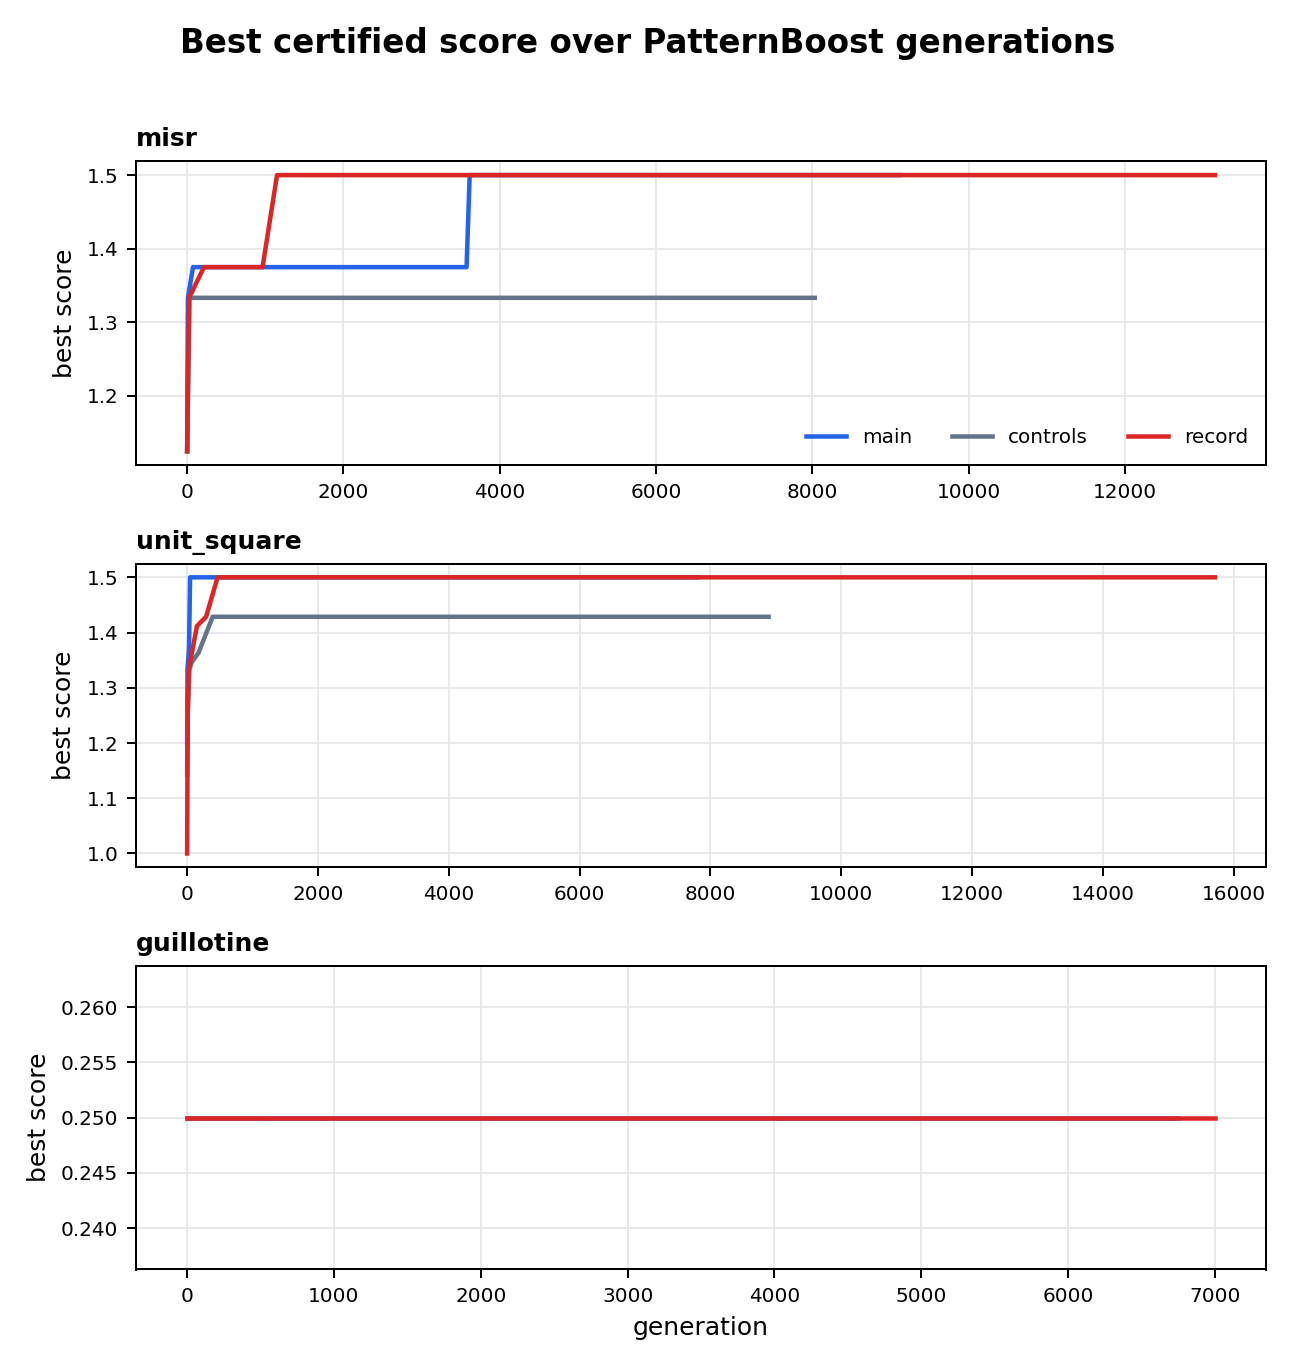
\includegraphics[width=0.95\textwidth]{fig_learning_curves.png}
\caption{Best certified score over PatternBoost generations for the final
submission run.  MISR and unit-square stabbing reach score $1.5$ in both the
main or record stages.  Guillotine remains at $0.25$ in the fresh final run.}
\label{fig:learning-curves}
\end{figure}

The compact source table for Figure~\ref{fig:learning-curves} is:
\begin{quote}
\artifact{docs/assets/final_submission_20260708_131302/plots/learning_curves_by_problem.csv}
\end{quote}
The full event streams remain on HPC and are not committed to the repository.

\clearpage
\section{Construction Gallery}

\begin{figure}[htbp]
\centering
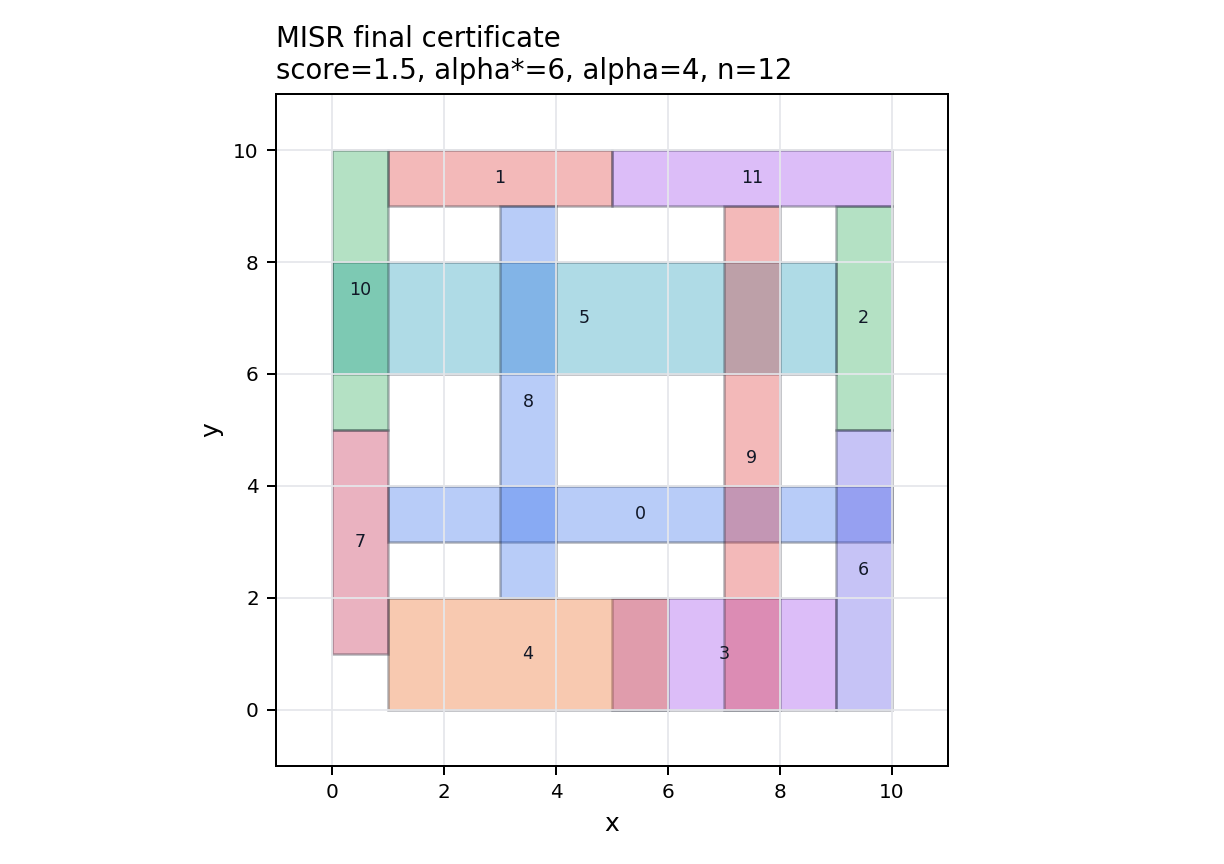
\includegraphics[width=0.82\textwidth]{fig_final_misr_1p5.png}
\caption{Final MISR certificate from the main matrix.  The exact verifier
computes $\alpha^*=6$ and $\alpha=4$, giving score $1.5$.}
\label{fig:misr-final}
\end{figure}

\begin{figure}[htbp]
\centering
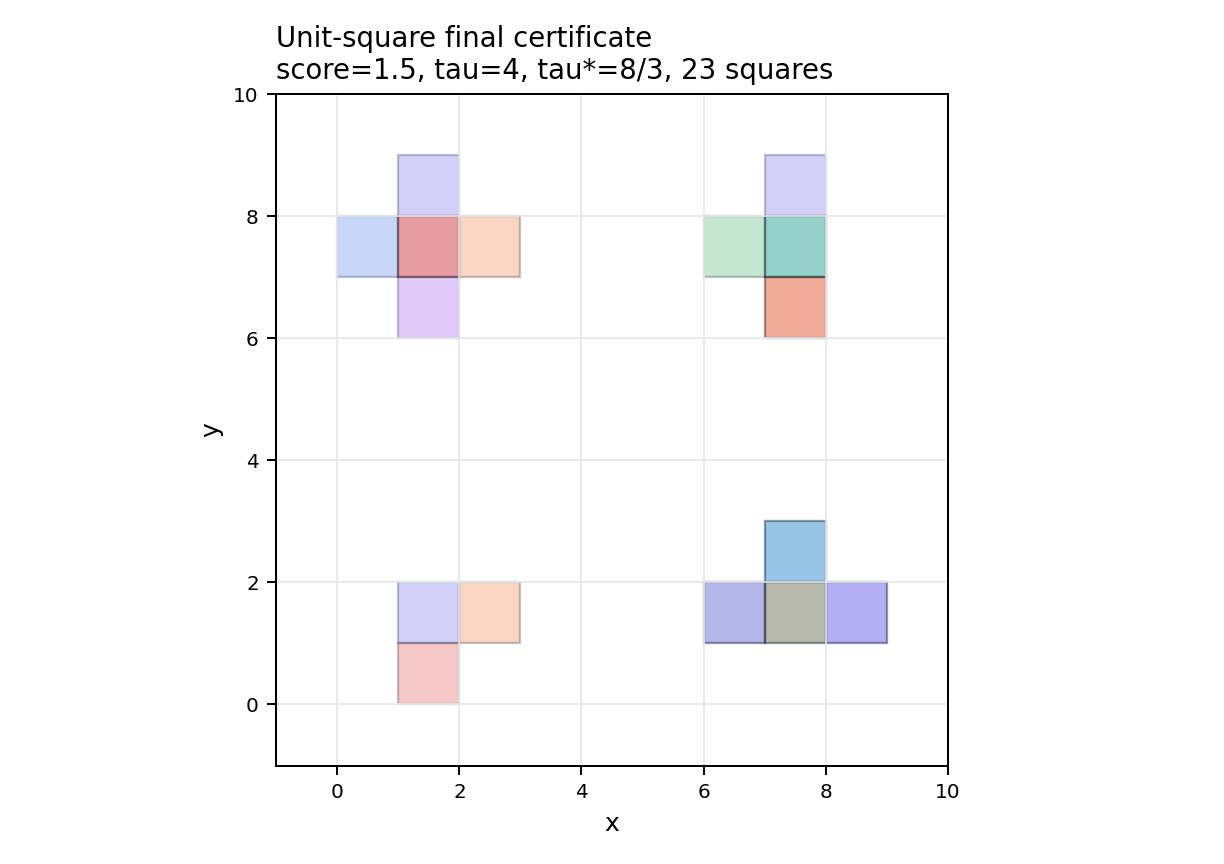
\includegraphics[width=0.82\textwidth]{fig_final_unit_square_1p5.png}
\caption{Final unit-square stabbing certificate from the main matrix.  The
exact set-cover verifier computes $\tau=4$ and $\tau^*=8/3$, giving score
$1.5$.}
\label{fig:unit-square-final}
\end{figure}

\begin{figure}[htbp]
\centering
\begin{minipage}{0.48\textwidth}
\centering
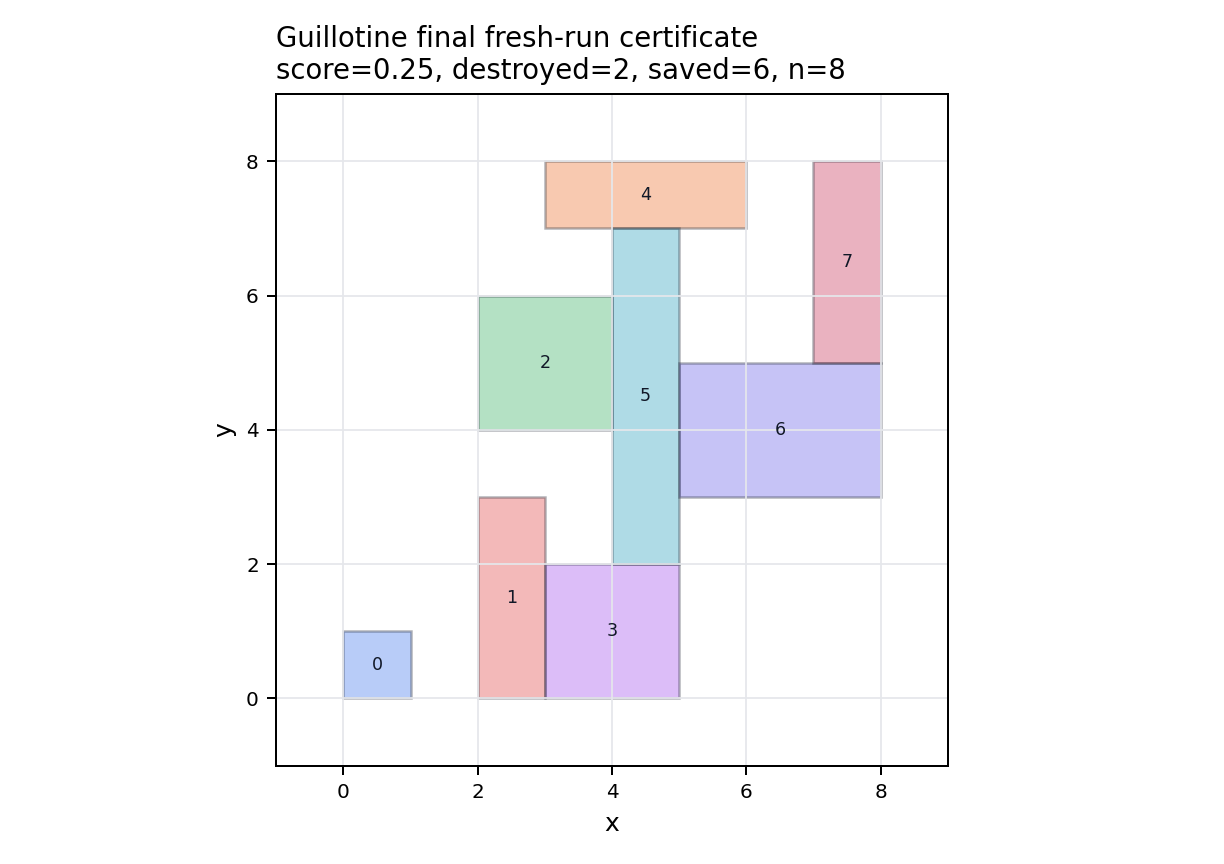
\includegraphics[width=\textwidth]{fig_final_guillotine_0p25.png}
\caption{Fresh final guillotine certificate, score $0.25$.}
\label{fig:guillotine-final}
\end{minipage}\hfill
\begin{minipage}{0.48\textwidth}
\centering
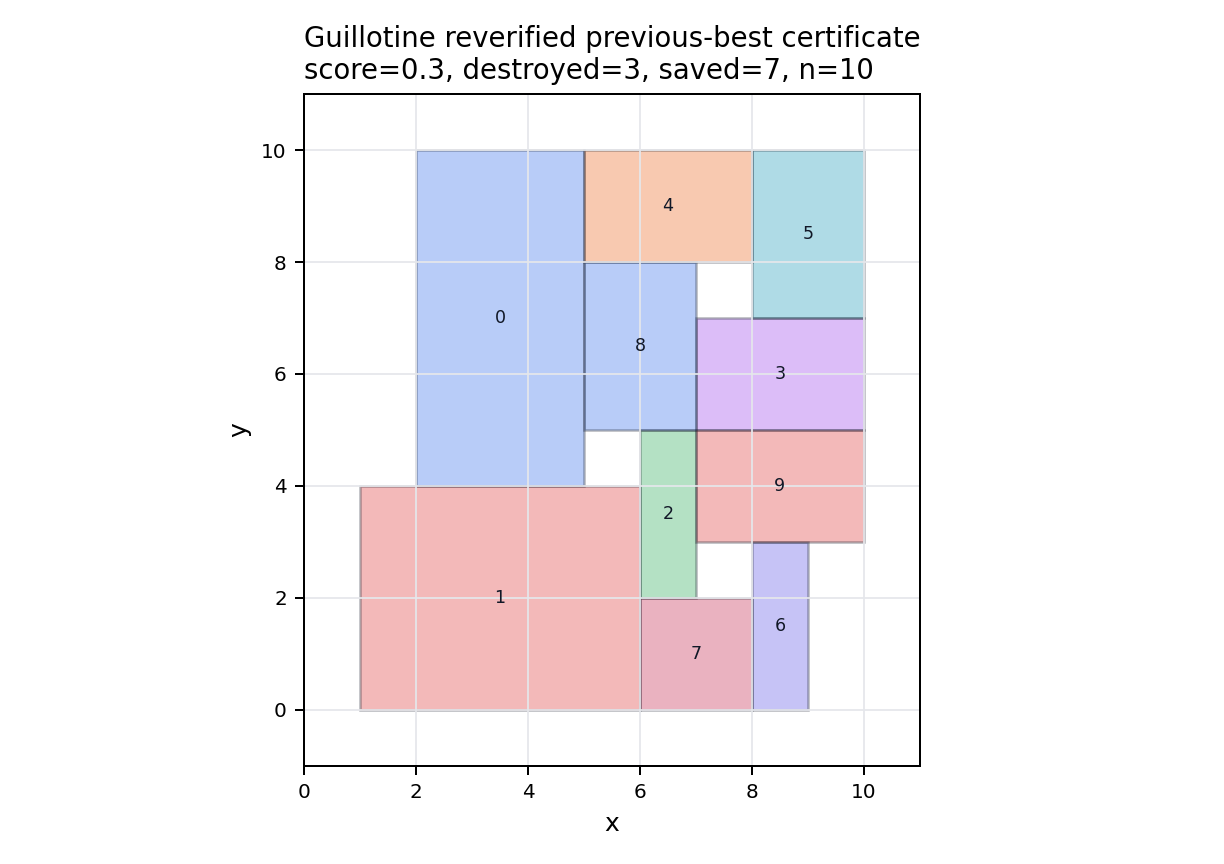
\includegraphics[width=\textwidth]{fig_reverified_guillotine_0p30.png}
\caption{Reverified previous-best guillotine certificate, score $0.3$.}
\label{fig:guillotine-prevbest}
\end{minipage}
\end{figure}

\section{Methodology by Problem}

\subsection{MISR}

For a rectangle family $\Rcal$, the reported score is
\[
        \score_{\rm MISR}(\Rcal)=\alpha^*(\Rcal)/\alpha(\Rcal),
\]
where $\alpha^*$ is the clique-LP optimum and $\alpha$ is the exact maximum
independent set.  The verifier recomputes the rectangle intersection graph,
LP value, integer optimum, maximal clique constraints, and certificate hash.

The final run confirms that the strongest current fresh certificates come from
structured sparse-conflict search.  The main winning row uses
\code{triangle\_free\_rect} with \code{program\_coeff\_pivot}; the record
follow-up ties it with \code{lp\_dual\_pivot}.  Both certify score $1.5$ on
12 rectangles.  This is stronger than the current controls, which stop at
$4/3$.

\subsection{Unit-Square Stabbing}

For a unit-square family $\Scal$, the reported score is
\[
        \score_{\rm stab}(\Scal)=\tau(\Scal)/\tau^*(\Scal),
\]
where $\tau$ is the exact minimum number of horizontal and vertical stabbing
lines and $\tau^*$ is the finite set-cover LP optimum over critical lines.

The final run certifies score $1.5$.  The main matrix reaches it with the
line-square incidence representation and the primal-dual line move; the record
follow-up ties it with line-square incidence plus coordinate mutation.  The
line-incidence representation is the useful ingredient: it exposes the
set-cover structure directly instead of relying only on raw coordinate
mutation.

\subsection{Guillotine}

For a disjoint rectangle packing, the exact verifier computes the maximum
number of rectangles that can be saved by a recursive guillotine cutting
strategy.  The reported score is
\[
        \score_{\rm guillotine}=1-\save/n
        =\text{destroyed}/n.
\]

The fresh final run certifies score $0.25$ in both main and record stages.
The stronger previous-best score $0.3$ is available only as a reverified
historical certificate in this repository snapshot.  The final record row that
matched the old $0.3$ configuration,
\[
\code{rect\_direct\_disjoint/packing\_resize/k\_subset\_nonseparability},
\]
ended with no best certificate under the final run.  In the older 36-hour run,
the $0.3$ certificate appeared late, after about 18 hours.  This suggests that
the construction family is viable but sparse under fresh stochastic search.

\section{Manuscript-Use Recommendations}

\begin{enumerate}
\item Use the fresh final run as the main reproducible experiment table:
MISR $1.5$, unit-square $1.5$, guillotine $0.25$.
\item If the manuscript wants the strongest available guillotine certificate,
quote $0.3$ only with the explicit provenance that it is a reverified
previous-best certificate, not rediscovered by the final fresh array.
\item Do not quote rows that failed audit because they lack
\code{best\_certificate\_path}.
\item Use Figure~\ref{fig:learning-curves} for training-progress charts and
Figures~\ref{fig:misr-final}--\ref{fig:guillotine-prevbest} for construction
illustrations.
\item Keep exploratory \code{epsilon\_net} and \code{graph\_separation}
results in an appendix or separate section.
\end{enumerate}

\section{Artifact Index}

\begin{longtable}{@{}p{0.30\textwidth}p{0.62\textwidth}@{}}
\caption{Repository artifacts for the final report.}\\
\toprule
Artifact & Path \\
\midrule
\endfirsthead
\toprule
Artifact & Path \\
\midrule
\endhead
\bottomrule
\endfoot
Main summary & \artifact{docs/assets/final_submission_20260708_131302/main_results/summary.csv} \\
Main audit & \artifact{docs/assets/final_submission_20260708_131302/main_results/audit/audit.json} \\
Controls summary & \artifact{docs/assets/final_submission_20260708_131302/control_results/summary.csv} \\
Controls audit & \artifact{docs/assets/final_submission_20260708_131302/control_results/audit/audit.json} \\
Record summary & \artifact{docs/assets/final_submission_20260708_131302/record_results/summary.csv} \\
Record audit & \artifact{docs/assets/final_submission_20260708_131302/record_results/audit/audit.json} \\
Final score table & \artifact{docs/assets/final_submission_20260708_131302/final_score_table.csv} \\
Learning curves & \artifact{docs/assets/final_submission_20260708_131302/plots/learning_curves_by_problem.csv} \\
Best certificates & \artifact{docs/assets/final_submission_20260708_131302/certificates/} \\
Best renderings & \artifact{docs/assets/final_submission_20260708_131302/renderings/} \\
Reverified guillotine $0.3$ & \artifact{docs/assets/final_submission_20260708_131302/reverified_previous_best/} \\
\end{longtable}

\end{document}
